\chapter{Løsningsimplementering}
Arbeidet i denne fasen går ut på å utrede en tiltaksplan og lage et forslag til hvordan dette skal implementeres. I den foregående fasen ble løsningene til rotårsaken identifisert til å være at alt materiale blir gratis og tilgjengelig på ett sted, tilby produkter fra selskap som universitetet får flest notiser fra, kurs for studenter i bruk av universitetsnettet og bytte av ISP på Sit-boligene. Kurs for studenter og bytting av ISP vil kunne stoppe NTNU fra å motta notifikasjoner for brudd på opphavsrett, men vil ikke nødvendigvis stoppe beboere fra å laste ned. 

\section{Tiltaksplan}
Gjennomføring av disse tiltakene vil i hovedsak administreres av universitetet og Sit.

\subsection{Alt av materiale blir gratis og tilgjengelig på ett sted}
Dette tiltaket vil fjerne rotårsaken helt og holdent. Alt materiale blir gratis, gitt ut på samme tid over hele verden og tilgjengelig på ett sted. Dette tiltaket har svært høy kost, men også høy nytte. Skolen må skaffe avtaler med alle produsenter og tilby det til studentene. Dette vil fjerne rotårsaken, men er urealistisk. 

\subsection{Tilby produkter fra selskap som universitetet får flest notiser fra}
Finne ut de mest populære selskapene som universitetet får notis fra, og skaffe en avtale med rettighetshaverne eller som er distributør for rettighetshaverene og gjøre dette tilgjengelig for studenter. Dette vil fjerne rotårsaken på at de laster ned fra dette selskapet. Dette har lav start kostnad som starter med å kartlegge hvilke firmaer som har høy frekvens av notiser. Kostnaden tilknyttet dette tiltaket er i hovedsak det å få til en avtale med rettighetshaverene, eller distributørene av materialet i Norge.

\subsection{Kurs for studenter i bruk av universitetsnettet}
Etablere et kurs for studenter om hvordan man skal bruke universitetsnettet. Nye studenter som kommer til NTNU vil ha som krav å gjennomføre kurset, som en del av signereingen av IT reglementet. Kurset vil avluttes med en test, for å se hvor mye av IT reglementet studenten har fått med seg. Denne testen kan muligens brukes i forbindelse med inititav/straff ettersom hvor godt studenten gjør det. Dette kurset kan bli for omfattende for hele universitetet og kan heller bare bli gitt til Sit leietakere. Dette prosjektet kan bli både tidkrevende og ha en høy kostnad, så vi foreslår for å begrense ressursbruken at dette prosjektet blir en mulig bacheloroppgave.   

\subsection{Sit bytter ISP}
Det å bytte ISP eller splitte studenthjemmene fra skolenettverket vil være en dyr og tidkrevende prosess, men dette kan være verdt å gjennomføre. Dette vil ikke fjerne rotårsaken til problemet, men vil flytte problemet vekk fra NTNU.


\section{Trediagram}
Trediagram benyttes for å lage en liste over aktiviteter som må gjennomføres for å implementere tiltaket. Trediagram er på et vis et utkast til en prosjektplan.

\subsection{Ønsket utbytte}
Ønsket utbytte ved å bruke trediagram er å få en liste over aktiviteter som må bli gjennomført for å innføre det spesifikke tiltaket.   

\subsection{Gjennomføring}
Dette verktøyet startet med å gruppere hovedtiltak til rotårsaken, deretter ble hver aktivitet som må gjennomføres for at tiltaket skal bli gjennomført gruppert. Disse underpunktene ble gruppert etter hvilken rekkefølge de skal bli implementert slik at tiltaket er mulig å gjennomføre. 

\subsection{Resultater}
Dette ga oss en fullstendig plan over hvilke aktiviteter som må gjennomføres for at tiltaket skal bli implementert. 

\begin{figure}[H] 
    \centering    
    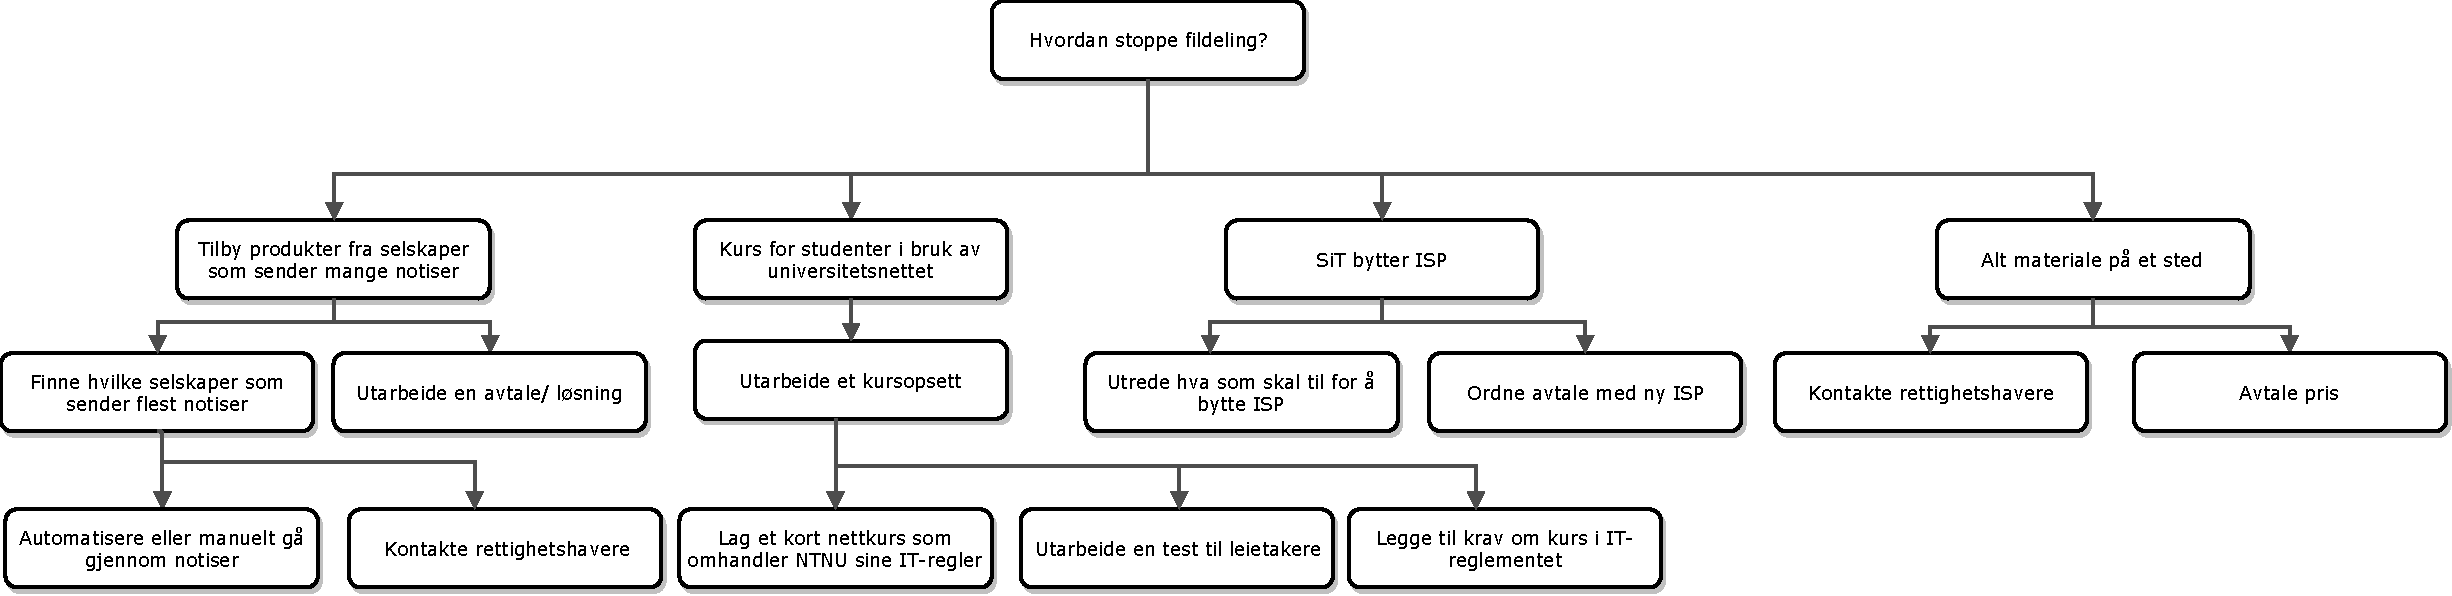
\includegraphics[scale=0.55, angle=90]{case_1/bilder/Tre-diagram.pdf}
    \caption[Trediagram til tiltak for case 1]{Løsningsimplementering}
    \label{fig:Tre-diagram}
\end{figure}

\subsection{Konklusjon av verktøy}
Dette verktøyet fungerte bra for å lage en plan til hvordan tiltakene skal bli implementert og hva som skal til for at tiltaket blir implementert. Trediagram er god måte å stykke opp arbeidsoppgavene for å skape en visuell prosess med oppgavene som må bli gjort for å nå målet.